\documentclass{ximera}

\addPrintStyle{..}

\begin{document}
	\author{Bart Lambregs}
	\xmtitle{Elastsiche potentiële energie}{}
    %\xmsource\xmuitleg


	%%%\section{Potentiële energie}

	Naast kinetische energie -- de energie geassocieerd met de beweging van een lichaam -- kunnen we een andere vorm van mechanische energie definiëren: de \textit{potentiële energie}. Dit is de energie geassocieerd met de plaats of configuratie van een lichaam. Een lichaam met kinetische energie heeft energie omdat het als gevolg van zijn beweging arbeid kan verrichten op een ander object. Kan een object arbeid verrichten als gevolg van zijn plaats, dan noemen we deze energie potentiële energie.
	
	Het leveren van arbeid op een voorwerp hoeft niet altijd te resulteren in een verandering van de kinetische energie. Bijvoorbeeld wanneer de arbeid van slechts \'e\'en van de krachten op een voorwerp wordt beschouwd en niet de arbeid door de resulterende kracht geleverd. De geleverde arbeid moet dan naar een andere vorm van energie gaan: potentiële energie. Bij het opwinden van een horloge bijvoorbeeld wordt de geleverde arbeid gebruikt om de veer samen te drukken. De veer kan zich daarna ontspannen en arbeid op de wijzers leveren.
	
	De vraag \textit{hoeveel} energie een voorwerp heeft, zal bij nader inzien enkel relatief kunnen worden bepaald. Is bijvoorbeeld de kinetische energie van een bekertje koffie op het tafeltje van de trein van Brussel naar Gent gelijk aan nul omdat het t.o.v. het tafeltje niet beweegt? Of is de kinetische energie verschillend van nul omdat het bekertje een snelheid heeft t.o.v iemand buiten de trein en dus, moest de trein plots stoppen, het bekertje verder zal vliegen en (veel opkuis-) arbeid kan leveren? En hoeveel energie heeft een blokje op een bepaalde hoogte? Zoveel als dat het arbeid kan leveren? Dat zal niet eenduidig te bepalen zijn. De geleverde arbeid tot op het tafeloppervlak, de grond of de bodem van de put die we vervolgens hebben gegraven is steeds verschillend. De geleverde arbeid, en dus de energie, is afhankelijk van het referentiepunt dat we nemen. In ieder geval moet de energie van een voorwerp afnemen met de hoeveelheid arbeid die het levert.
	
	%Potentiële energie is echter niet in alle gevallen te
	%definiëren. In namelijk niet alle gevallen is de mogelijk te
	%leveren hoeveelheid arbeid eenduidig bepaald.
	
	%%%\newpage
	
	\subsection{Elastische potentiële energie}\label{elastische
	potentiele energie}
	
	We hernemen het voorbeeld van de veerkracht (\ref{voorbeeld Hooke}).
	\begin{image}
	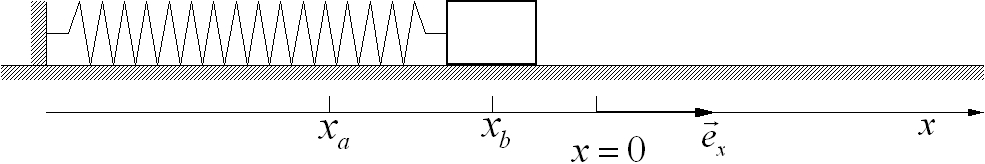
\includegraphics[width=0.8\textwidth ,angle=0]{elastische_energie}
	\end{image}


	%%%\newline

	Hier vonden we dat de hoeveelheid arbeid door de veerkracht geleverd
	bij een verplaatsing van $x_a$ naar $x_b$ gegeven wordt door:
	\begin{eqnarray*}
	W&=&\frac{1}{2}kx_ a^2-\frac{1}{2}kx_ b^2
	\end{eqnarray*}
	De geleverde arbeid kan geschreven worden als het verschil van de uitdrukking $\frac{1}{2}kx^2$ geëvalueerd in begin- en eindpunt. De waarde van de uitdrukking neemt af met de hoeveelheid arbeid die is geleverd. We kunnen de uitdrukking dus interpreteren als de hoeveelheid energie die de veer op een bepaald punt, een bepaalde plaats, bezit. Dat wat immers verloren gaat aan energie -- de oorspronkelijke energie min de overblijvende energie -- moet door de veer worden geleverd als arbeid. We noemen de uitdrukking de \textit{elastiche potentiële energie} van een veer:
	\begin{eqnarray}
	E_p&=&\frac{1}{2}kx^2
	\end{eqnarray}
	De geleverde arbeid kunnen we vervolgens schrijven als
	\begin{eqnarray*}
	W&=&E_{p,a}-E_{p,b}\,=\,-(E_{p,b}-E_{p,a})\\
	&\Updownarrow&\\
	W&=&-\Delta E_p
	\end{eqnarray*}
	Hierin is $\Delta E_p$ de verandering van potentiële energie: $\Delta E_p=E_{p,\rm eind}-E_{p,\rm begin}$. Als de veer arbeid verricht dan gaat dat ten koste van haar potentiële energie: is de geleverde arbeid $W$ positief, dan moet er een afname van de potentiële energie zijn (de verandering $\Delta E_p$ moet negatief zijn). Opnieuw: de hoe\-veel\-heid geleverde arbeid komt overeen met het verlies in potentiële energie tussen begin- en eindpunt. Is de verandering van de potentiële energie $\Delta E_p$ positief dan is de geleverde arbeid negatief. Negatieve arbeid betekent dat i.p.v. het leveren van arbeid (het weggeven van energie), er van elders energie wordt toegevoegd en wordt omgezet in potentiële energie.
	
\end{document}
